\documentclass[mathserif,11pt]{beamer}

\usepackage{pdfpages}
\usepackage{tex/fontawesome} % nice glyphs

% Turn off the ugly navigation symbols.
\setbeamertemplate{navigation symbols}{}

% Margins and whatnot.
\setbeamersize{text margin left=1em,text margin right=1em}

% Hoefler Text as the main text font; need to make sure it's happy
% using serif though...
\usepackage{fontspec}
\usefonttheme{serif}
\defaultfontfeatures{Mapping=tex-text} % enable -- / --- / `` / ''
\setmainfont{Hoefler Text}
\setsansfont[BoldFont=Oswald Bold,ItalicFont=Oswald Light]{Oswald}
\newcommand{\amp}{{\fontspec[Alternate=1]{Hoefler Text}\&}}
\newcommand{\QQ}{{\fontspec[Alternate=2]{Hoefler Text}Q}}

\usepackage{tabularx}
\usepackage{array}

\definecolor{verydarkgrey}{HTML}{001112}
\definecolor{fdarkblue}{HTML}{232747}
\definecolor{lightgrey}{HTML}{eeeeee}
\definecolor{grey}{rgb}{0.5, 0.5, 0.5}
\definecolor{darkgreen}{rgb}{0, 0.4, 0} % same as "darkgreen" in R

\setbeamerfont{frametitle}{size=\large}
\setbeamercolor{frametitle}{fg=black}
\setbeamercolor{titleline}{bg=black}
\setbeamercolor{title}{fg=fdarkblue}
\setbeamercolor*{date in head/foot}{fg=verydarkgrey}
\setbeamercolor{item}{fg=fdarkblue}
\setbeamerfont{item}{series=\bfseries}
% Never used, but this is nice.
\setbeamertemplate{itemize subitem}{\normalsize --}

% \useoutertheme{new}

\makeatletter  %Sets category code: http://tex.stackexchange.com/questions/8351/what-do-makeatletter-and-makeatother-do
\usepackage{dashrule}
\defbeamertemplate*{frametitle}{mine}[1][left]
{
  % Increase width of title box
  \@tempdima=\textwidth%
  \advance\@tempdima by\beamer@leftmargin%
  \advance\@tempdima by\beamer@rightmargin%
  %
  \begin{beamercolorbox}[sep=0.3cm,#1,wd=\the\@tempdima]{frametitle}
    \usebeamerfont{frametitle}%
    \vbox{}\vskip-1ex\vspace{.5ex}
    \strut\hspace{1ex}\insertframetitle\strut\par%
    \vskip-1.5ex%
    \hspace{\fill}\hdashrule{\textwidth}{.075ex}{.075ex .2ex}\hspace{\fill}
    \par\nointerlineskip \vspace{\baselineskip}
  \end{beamercolorbox}%
  \nointerlineskip%
  \vspace{-1ex}
}

\setbeamercolor*{date in head/foot}{bg=black,fg=white}




\usepackage{tikz}
\usetikzlibrary{positioning}
\usetikzlibrary{calc}
\usetikzlibrary{arrows,positioning, decorations, decorations.text}

% Define new environment for overlaying transparent text box, eg.g. for title
\usepackage[framemethod=tikz]{mdframed}
\newmdenv[tikzsetting={draw=black,fill=white,fill opacity=0.7, line width=4pt, rounded corners, inner sep=10pt, inner ysep=10pt},backgroundcolor=none,leftmargin=0,rightmargin=0,innertopmargin=4pt,skipbelow=\baselineskip,%
skipabove=\baselineskip]{TitleBox}

% macro for small text at lower right of screen, e.g. links
\usepackage[overlay,absolute]{textpos}
\newcommand\FrameText[1]{
  \begin{textblock*}{\paperwidth}(0pt,.98\textheight)
    \raggedleft \small  #1\hspace{.5em}
  \end{textblock*}}

% some formatting options for green blue slide
\tikzstyle{greenblue_bodytext} = [text width=.45\paperwidth,text badly ragged,  rounded corners, inner sep=10pt, inner ysep=10pt, fill=white, line width=2pt]

% Defines a command to make two new slides with different backgorunds,
% place two text boxes on page n top left and bottom right,

\newcommand{\greenblueslide}[6]{%
\begin{frame}[empty]
   \begin{tikzpicture}[remember picture,overlay]
     \node at (current page.center) {
       \includegraphics<1>[width=\paperwidth]{#1}
       \includegraphics<2>[width=\paperwidth]{#4}
     };
     \node[draw,anchor=north west, greenblue_bodytext, draw= green] at
       ($(current page.north west) + (.05\paperwidth, -.1\paperheight)$)
       {{\bf Plants: }\\ {\small #2}};

     \only<2>{
     \node[draw,anchor=south east, greenblue_bodytext, draw=blue] at
       ($(current page.south east) - (.05\paperwidth, -.1\paperheight)$)
       {{\bf Marine: }\\ {\small #5}};
       }
   \end{tikzpicture}
   \only<1>{ \FrameText{ {\color{grey} #3}}}
   \only<2>{ \FrameText{ {\color{grey} #6}}}
\end{frame}
}

\newcommand{\traitsummary}[9]{

\tikzstyle{boxStyle1}=[anchor = center, rectangle, rounded corners, thick, inner sep=4pt, inner ysep=4pt, align = center, fill =white, text width = 3cm]
\tikzstyle{boxStyle2}=[boxStyle1, text width = 8cm]

% define styles - lines
\tikzstyle{lineStyle1}=[shorten <=2pt, shorten >=2pt]

  % anchor
  \node[] at ($(current page.center) + (0, 3cm)$) (middle){};
  % top row
   \node[boxStyle1, left = 3cm of middle.center, text = darkgreen] (low) { #1  };
   \node[boxStyle1, right = 3cm of middle.center, text = darkgreen] (high) { #3 }
      edge [<->, line width = 5pt, lineStyle1, draw=darkgreen!50]                  (low);
  \node[boxStyle1 , draw = black, text width = 3cm] at (middle) {\large #2};
  % second row
  \node[boxStyle2, below = 0.8cm of middle.center, text = black!50] (middle2) {\small (direct physiological trade-off)};
   \node[boxStyle1, left = 3cm of middle2.center] (low2) {\small #4};
   \node[boxStyle1, right = 3cm of middle2.center] (high2) {\small #5};
  % 3rd row
  \node[boxStyle2, below =0.8cm of middle2.center, text = black!50] (middle3) {\small (functional outcome)};
   \node[boxStyle1, left = 3cm of middle3.center, text = black] (low3) {\small #6};
   \node[boxStyle1, right = 3cm of middle3.center, text = black] (high3) {\small #7};
 % 4th row
  \node[boxStyle2, below =0.8cm of middle3.center, text = black!50] (middle4) {\small (demographic outcome)};
   \node[boxStyle1, left = 3cm of middle4.center, text = black] (low4) {\small #8};
   \node[boxStyle1, right = 3cm of middle4.center, text = black] (high4) {\small #9};

}


% From Rich - macro for???
\makeatother   % Sets category code: http://tex.stackexchange.com/questions/8351/what-do-makeatletter-and-makeatother-do
\usepackage{relsize}
\newenvironment{tframe}{
  \begin{frame}[plain]
    \begin{tikzpicture}[remember picture,overlay]
      \node[at=(current page.center)] {
        \includegraphics[width=\paperwidth]{pics/purple-gradient-background}
      };
    \end{tikzpicture}
    \color{white}
    \sf\relsize{3}}
    {\end{frame}}

% Colours come from colour brewer
\usepackage{xcolor}
\definecolor{b-blue}{HTML}{6baed6}
\definecolor{b-darkgrey}{HTML}{2D2D2D}
\definecolor{b-grey}{HTML}{969696}
\definecolor{b-purple}{HTML}{9e9ac8}
\definecolor{b-green}{HTML}{74c476}
\definecolor{b-pink}{HTML}{e377c2}
\definecolor{b-orange}{HTML}{FD8D3C}

\usepackage{relsize}

\usepackage{fontspec}
\defaultfontfeatures{Mapping=tex-text} % enable -- / --- / `` / ''
\setsansfont[ItalicFont={* Light},BoldItalicFont={* ExtraLight}]{Yanone Kaffeesatz}
\setmonofont[Scale=0.75]{Bitstream Vera Sans Mono}

% Neutralise underscores, since we don't use them apart for in URLs
\catcode`_=12
\begingroup\lccode`~=`_\lowercase{\endgroup\let~\sb}
\mathcode`_="8000



\newcommand{\hrefp}[2]{\href{#1://#2}{#2}}
\newcommand{\twitterhandle}[1]{\href{https://twitter.com/#1}{#1}}
\newcommand{\plant}{\texttt{plant}}

\title{Introduction to the {\plant} package for R\\(insert custom title slide)}
\date{}
\author{}

%----------------------------------------------------------------------------------------
\begin{document}
%-----------------------------------------------------------------------------------

\setbeamertemplate{background}
{
\includegraphics[width=\paperwidth,height=\paperheight,keepaspectratio]{pics/background.png}}

 \begin{frame}[plain]
 \vspace{10em}
 \begin{TitleBox}
  {\LARGE \inserttitle} \vskip3pt
  {\footnotesize \insertdate\vskip6pt
  \insertauthor }
 \end{TitleBox}
 \end{frame}

% NOTES
\begin{frame}[plain]

\begin{tikzpicture}[remember picture, overlay]%
  \node[anchor=north, align=center] at
    ($(current page.north) + (0cm, 0.2cm)$) {
    
\includegraphics[width=1.0\paperwidth]{pics/MEE}};

  \node [anchor=north, align=left, text width =10.5cm] at
    ($(current page.center) + (0, 0.25\paperheight)$) {%

  {\footnotesize
  {\normalsize \FA \faBook} \,\,  Falster, FitzJohn, Brännström, Dieckmann, Westoby (2016) {\bf plant: A package for modelling forest trait ecology and evolution}. \emph{Methods in Ecology and Evolution} XX: XXX. doi: \href{http://doi.org/10.1111/2041-210X.12525}{10.1111/2041-210X.12525}\\

    \vspace{1.5em}
  {\normalsize \FA \faDesktop} \,\, An ``Application note'' about a new package for R, called ``{\plant}''

  \vspace{1.5em}
  {\normalsize \FA \faGithub} \,\,  \hrefp{https}{github.com/traitecoevo/plant} }
  };

  \node[anchor=north, align=center] at
    ($(current page.center) + (0, -0.15\paperheight)$) {
    \includegraphics[width=0.8\paperwidth]{snippets/plant_install.pdf}
    };
\end{tikzpicture}

\end{frame}

% NOTES
\begin{frame}[plain]
\begin{tikzpicture}[remember picture, overlay]
  \node[anchor=north, align=center] at
    ($(current page.north)+ (0cm, 0.2cm)$) {
    \includegraphics[width=1.1\paperwidth]{downloads/BCI.jpg}};

  \node[anchor = center, align=left] at ($(current page.center) + (0cm, -4cm)$) {
 \resizebox{.9\paperwidth}{!}{%
 \color{white} A simulation model for exploring demographic phenomena}
  };
\end{tikzpicture}
\end{frame}

% NOTES
\begin{frame}{Individual-based model $\rightarrow$ start with single plant}
  \begin{center}
   \includegraphics<1>[height=.8\textheight]{figures/plantmodel-1}
  \end{center}
\end{frame}

% NOTES
% 1. *A plant* has a size (height, allometric scaling for
%    other sizes), probability of dying and a rate of seed production.
% 2. All these rates are functions of *total carbon assimilation*,
%    which is a function of the plant's leaf area distribution (canopy
%    shape) and the light environment.
% 3. The carbon fixed is then assigned to maintenance, growth and
%    reproduction.  Your probability of mortality depends inversely on
%    the amount of photosynthesis you do.
% 4. (The key ingredient is how much carbon you fix; we consider light
%    primarily as the limiting resource)

\begin{frame}{Individual-based model $\rightarrow$ rules about plant function}
  \begin{center}
   \includegraphics<1>[height=.8\textheight]{figures/plantmodel-7}
  \end{center}
\end{frame}


% NOTES:
% The light environment is derived by summing over all the leaf
% area distributions of all individuals -- it also varies over time
% and emerges from the model.  It provides a strong feedback between
% all individuals in the model.
%
% [Plants grow in the context of a forest; how much light you get
% depends on who grows around you and how big they are; but that
% depends on who grows around those plants, and so on.  This is the
% key feedback]

\begin{frame}{Competition due to shading}
  \begin{center}
    \includegraphics<1>[height=.8\textheight]{figures/lightenv-1}
    \includegraphics<2>[height=.8\textheight]{figures/lightenv-2}
    \includegraphics<3>[height=.8\textheight]{figures/lightenv-3}
  \end{center}
\end{frame}

% NOTES:
\begin{frame}{Plants compete within a patch}
  \begin{center}
   \includegraphics<1>[height=.8\textheight]{figures/patch-2}
  \end{center}
\end{frame}

% NOTES:
\begin{frame}{Many patches $\rightarrow$ a metapopulation}
  \begin{center}
   \includegraphics<1>[height=.8\textheight]{figures/patch-3}
  \end{center}
\end{frame}
% NOTES:
\begin{frame}{Multiple species (defined via traits) $\rightarrow$ a metacommunity}
  \begin{center}
   \includegraphics<1>[height=.8\textheight]{figures/patch-4}
  \end{center}
\end{frame}

% NOTES:
\begin{frame}{Key methodological advances making {\plant} possible}

  \begin{tikzpicture}[remember picture, overlay]%
    \node [anchor=north, align=left] at
    ($(current page.center) + (0, 3cm)$) {%
  {\small

  \begin{tabular}{cl}
  1970-1990 & Stochastic gap models \\
            & {\footnotesize \; \color{grey} $\rightarrow$ e.g. \href{http://doi.org/10.2307/2258570}{Botkin 1972}, \href{https://books.google.com.au/books/about/A_theory_of_forest_dynamics.html?id=q5vwAAAAMAAJ&redir_esc=y}{Shugart 1984}} \\[2ex]
  1985-2000 & Approximation with partial differential equations (PDEs) \\
            & {\footnotesize \; \color{grey} $\rightarrow$  \href{https://books.google.com.au/books?id=MXz1CAAAQBAJ}{Metz \& Diekmann 1986}, \href{http://doi.org/10.2307/2261230}{Kohyama 1993}, \href{http://doi.org/10.1890/0012-9615(2001)071[0557:AMFSVD]2.0.CO;2}{Moorcroft \emph{et al.} 2001} }  \\[2ex]
  2000-2015 & Generic plant physiology, function driven by traits \\
            & {\footnotesize \; \color{grey} $\rightarrow$  \href{http://doi.org/10.1890/0012-9615(2001)071[0557:AMFSVD]2.0.CO;2}{Moorcroft \emph{et al.} 2001}, \href{http://doi.org/10.1146/annurev.ecolsys.33.010802.150452}{Westoby \emph{et al.} 2002}, \href{http://doi.org/10.1111/j.1365-2745.2010.01735.x}{Falster \emph{et al.} 2011}} \\[2ex]
  2005-2015 & New numerical methods for solving PDEs \\
            & {\footnotesize \; \color{grey} $\rightarrow$ \href{http://doi.org/10.1016/j.apnum.2004.01.007}{Angulo \emph{et al.} 2004}, \href{http://doi.org/10.1016/j.camwa.2014.04.009}{2014} }\\[2ex]
  2010-2015 & New techniques for packaging, testing \& distributing code \\
            & {\footnotesize \; \color{grey} $\rightarrow$  \href{http://www.rcpp.org/}{Rcpp}, \href{https://github.com/richfitz/RcppR6}{RcppR6}, \href{https://github.com/traitecoevo/plant}{github}, \href{https://travis-ci.org/traitecoevo/plant}{Travis CI}} \\[4ex]
  {\plant} & One in a family of related models\\
   & {\footnotesize \; \color{grey} $\rightarrow$ e.g. \href{https://github.com/EDmodel/ED2}{ED}, \href{http://formind.org/model/}{FORMIND},  \href{http://iis4.nateko.lu.se/lpj-guess/}{LPJ-GUESS} } \\
  \end{tabular}
  }
};
\end{tikzpicture}
\end{frame}


\begin{frame}{Speed of C++ with flexibility of R  {\color{b-pink} {\FA \faHeart \faHeart \faHeart}} }
\begin{tikzpicture}[remember picture, overlay]%
  \node[anchor=north, align=center] at
    ($(current page.center) + (0, 0.3\paperheight)$) {
    \includegraphics[width=.9\paperwidth]{snippets/plant_package}};
  \end{tikzpicture}
\end{frame}


\begin{frame}{4 options for using {\plant}}
\begin{tikzpicture}[remember picture, overlay]%
  \node[anchor=north, align=center] at
    ($(current page.center) + (0, 0.3\paperheight)$) {
     \includegraphics[width=.9\paperwidth]{snippets/plant_options}
    };
  \end{tikzpicture}
\end{frame}% NOTES:
% 1. Consider species as vectors of traits
% 2. Fitness is the expected number of offspring per individual, but
%    varies depending on the number and types of other individuals.
% 3. Throw in a bunch of seeds, and see how many seeds each seed
%    produces.  Consider traits to be fixed through this part.  This
%    is our "ecological black box"
\begin{frame}{``Demography beyond the population'' -- e.g. fitness}
  \begin{center}
    \includegraphics<1>[height=.8\textheight]{figures/fitness-3}
    \includegraphics<2>[height=.8\textheight]{figures/fitness-4}
  \end{center}
\end{frame}

\begin{frame}{{\plant} integrates seed production over entire life-cycle}
  \begin{center}
    \includegraphics<1>[height=.8\textheight]{figures/paper-f3.pdf}
  \end{center}
\end{frame}

% NOTES:
% 1. A seed is the natural place to census how types are doing.
% 2. Seeds are discrete things, and we can count them up.
% 3. A plant is simply a seeds way of making more seeds, and we can
%    largely ignore them when considering how species are doing (how
%    important is a large plant that will never reproduce).
% 4. However, they are fairly important ecologically...
% 5. To produce a new seed, the seed must
%    - germinate
%    - grow to maturity (and bigger plants make more seed)
%    - have enough spare energy to go into reproduction
% 6. So most of the ecology will focus on the plant.
% 7. But this cycle really is all that is in the black box.


\begin{frame}{Quantify trait-based niche differentiation (stable coexistence)}
  \begin{center}
    \includegraphics<1>[height=.8\textheight]{figures/paper-f5}
  \end{center}
\end{frame}

\begin{frame}\frametitle{Thanks to collaborators}

  \begin{tikzpicture}[remember picture, overlay]%
    \node [anchor=north, align=left] at
    ($(current page.center) + (0, .37\paperheight)$) {%
    {\footnotesize
      \begin{tabular}{c >{\color{black}}l  c >{\color{black}}l }
        \raisebox{-.03\paperheight}{%
          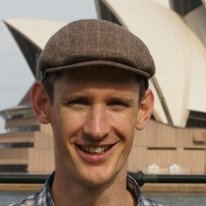
\includegraphics[height=.12\paperheight]{pics/people/FitzJohn}}&
        Rich FitzJohn  &
        \raisebox{-.03\paperheight}{%
          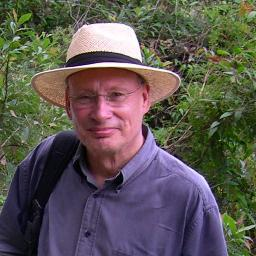
\includegraphics[height=.12\paperheight]{pics/people/Westoby.jpeg}}&
       Mark Westoby  \\
       & & & \\
        \raisebox{-.03\paperheight}{%
          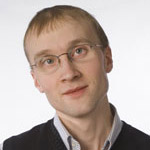
\includegraphics[height=.12\paperheight]{pics/people/Brannstrom}}&
        Åke Brännström &
        \raisebox{-.03\paperheight}{%=
          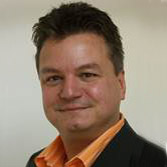
\includegraphics[height=.12\paperheight]{pics/people/Dieckmann}}&
        Ulf Dieckmann\\
     \end{tabular}
      }
  };
   \node [anchor=north, align=left, text width =10.5cm] at
    ($(current page.center) + (0, 0\paperheight)$) {%

  {\footnotesize
  {\normalsize \FA \faBook} \,\,  Falster, FitzJohn, Brännström, Dieckmann, Westoby (2016) {\bf plant: A package for modelling forest trait ecology and evolution}. \emph{Methods in Ecology and Evolution} XX: XXX. doi: \href{http://doi.org/10.1111/2041-210X.12525}{10.1111/2041-210X.12525}

  \vspace{1em}
  {\normalsize \FA \faAlignJustify}  \,\,  \href{xxx}{xxx}

  \vspace{1em}
  {\normalsize \FA \faGithub} \,\,  \hrefp{https}{github.com/traitecoevo/plant}, \hrefp{https}{github.com/traitecoevo/plant\_paper}

  \vspace{1em}
  {\normalsize \FA \faTwitter}  \,\,  \twitterhandle{adaptive\_plant}, \twitterhandle{rgfitzjohn}
  }
  };
  \end{tikzpicture}
\end{frame}

\end{document}
